\documentclass{IEEEtran}

\usepackage{cite}
\usepackage{amsmath,amssymb}
\usepackage{graphicx}
\usepackage{textcomp}
\usepackage{xcolor}
\usepackage{booktabs}
\usepackage{multirow}
\usepackage{array}
\usepackage[hidelinks]{hyperref}

\begin{document}

\title{\textbf{Hybrid EfficientNet-B2 and SVM Framework for Automated Solar-Panel Dust Detection with Explainable AI}}

\author{
Aditya Shirsatrao\\
Department of Artificial Intelligence and Data Science\\
N K Orchid College of Engg \& Tech, Solapur, MH, India\\
Email: adityashirsatrao007@gmail.com
}

\maketitle

\begin{abstract}
This paper presents an automated, explainable framework for detecting dust accumulation on photovoltaic (PV) panels from a single RGB image. We propose a hybrid architecture that couples a frozen EfficientNet-B2 convolutional encoder with a support vector machine (SVM) head: the backbone extracts a 1,408-dimensional global-average-pooled feature vector, which a radial-basis-function SVM classifies into \emph{clean} or \emph{dirty}. The frozen backbone avoids overfitting on modest per-source datasets while the SVM head delivers a margin-based, well-calibrated decision boundary. To make every prediction auditable, the framework includes a multi-method explainability module (Grad-CAM, Score-CAM, Integrated Gradients, SHAP, and LIME) that localises the dust evidence and exposes the texture channels driving each decision. Evaluated on a merged multi-source corpus of 3,787 panel images (3,029 train / 377 validation / 381 test), the model achieves \textbf{90.29\%} test accuracy, \textbf{0.9596} AUC-ROC, and \textbf{86.38\%} 5-fold cross-validation accuracy with only 7.77M backbone parameters. Crucially, the model also generalises to two fully independent external datasets at 98.24\% and 99.74\% accuracy, demonstrating that the learned representation is not tied to a single acquisition source. An ablation across three backbones shows MobileNetV3-Large reaches 88.71\% at the smallest parameter budget (3.00M) while ResNet50 matches the deployed model at 90.29\% (23.59M), confirming the hybrid CNN+SVM paradigm is robust and efficient for field deployment.
\end{abstract}

\begin{IEEEkeywords}
automated dust detection, EfficientNet-B2, support vector machine, hybrid feature-space classification, solar photovoltaic, explainable AI (Grad-CAM, Score-CAM, Integrated Gradients, SHAP, LIME)
\end{IEEEkeywords}

\section{Introduction}

Dust accumulation on PV panels reduces power output and accelerates degradation, motivating condition-based rather than schedule-based cleaning. Automated visual inspection from a single image is therefore an active research problem. Modern compound-scaled convolutional networks such as EfficientNet~\cite{tan2019efficientnet} extract powerful transferable features, and when paired with a margin-based classifier such as an SVM they often generalise better than an end-to-end softmax head on small, noisy, field-acquired datasets~\cite{bassil2025efficient}. A detector is only trustworthy, however, once it can explain itself; we therefore couple predictive accuracy with a multi-method explainability branch that makes every audit verifiable by a human operator.

The main contributions of this paper are:
\begin{enumerate}
\item An EfficientNet-B2 feature encoder paired with an RBF-SVM head for binary dust detection (clean vs dirty), achieving \textbf{90.29\%} accuracy on a 3,787-image merged corpus with only 7.77M backbone parameters, and generalising to independent external datasets at 98.24\%/99.74\%.
\item A two-phase training strategy (frozen feature extraction followed by optional fine-tuning of the last 30\% of the backbone) that establishes when fine-tuning helps and when the frozen representation is already sufficient.
\item A backbone ablation across EfficientNet-B2, MobileNetV3-Large, and ResNet50, showing MobileNetV3-Large attains 88.71\% at the lowest parameter cost (3.00M) while ResNet50 matches the deployed model at 90.29\% (23.59M).
\item A unified explainability module fusing Grad-CAM, Score-CAM, Integrated Gradients, SHAP feature attributions, and LIME, delivering auditable and repeatable dust audits.
\end{enumerate}

The remainder of this paper is organised as follows. Section~II reviews related work. Section~III details the dataset, architecture, training strategy, and explainability pipeline. Section~IV reports experimental results, the backbone comparison, and cross-dataset generalisation. Section~V concludes with findings and future work.

\section{Literature Review}

\subsection{Deep Learning Foundations}
Krizhevsky et al. established deep CNNs for image classification~\cite{krizhevsky2012imagenet}. He et al. proposed ResNets with skip connections~\cite{he2016deep}. Simonyan and Zisserman showed that a deep stack of small $3\times3$ convolutions (VGG16) transfers well~\cite{simonyan2015very}. Tan and Le introduced EfficientNet with compound scaling of width, depth, and resolution, achieving strong accuracy with fewer parameters~\cite{tan2019efficientnet}. These works underpin the encoders used in our detector.

\subsection{Solar Soiling Detection}
Onim et al. introduced SolNet, a CNN for panel dust detection, reporting 98.2\% accuracy on a 2,231-image benchmark~\cite{onim2023solnet}. Alatwi et al. evaluated 20 pretrained encoders with SVM heads, with DenseNet-169 + linear SVM reaching 86.79\%~\cite{alatwi2024deep}. Bassil et al. combined deep encoders with tree-based heads to quantify dust severity, reaching 97\%~\cite{bassil2025efficient}. Kourtiche et al. recently surveyed multi-task dust monitoring and cleaning optimisation frameworks~\cite{kourtiche2026}. These systems often offer limited explanation of their predictions.

\subsection{Hybrid Feature-Space Classifiers}
Support vector machines learn maximum-margin boundaries that generalise well on moderate feature spaces~\cite{cortes1995support}. Recent work confirms that a pretrained CNN encoder concatenated with an SVM yields higher stability than softmax heads on small, noisy datasets~\cite{bassil2025efficient}. Our framework adopts this two-stage paradigm, coupling EfficientNet-B2 features with an RBF-kernel SVM.

\subsection{Efficient Mobile Deployment}
Howard et al. introduced MobileNets using depthwise separable convolutions~\cite{howard2017mobilenets}; Sandler et al. devised MobileNetV2 with inverted residuals~\cite{sandler2018mobilenetv2}. EfficientNet's compound scaling~\cite{tan2019efficientnet} offers a principled alternative with strong accuracy/size trade-offs, motivating the backbone comparison in this work.

\subsection{Explainable AI for Vision}
Selvaraju et al. proposed Grad-CAM using gradients into the final convolutional layer~\cite{selvaraju2017grad}. Wang et al. introduced Score-CAM, a gradient-free variant~\cite{wang2020score}. Sundararajan et al. developed Integrated Gradients satisfying the completeness axiom~\cite{sundararajan2017axiomatic}. Lundberg and Lee unified attributions under Shapley values in SHAP~\cite{lundberg2017unified}. Ribeiro et al. introduced LIME for model-agnostic local explanations~\cite{ribeiro2016should}. These methods form the interpretability backbone of our audit.

\section{Methodology}

\subsection{Dataset}
We assemble a merged corpus of 3,787 RGB images of PV panels labelled as \emph{clean} or \emph{dirty}, drawn from three publicly available solar-panel dust sources: a Kaggle PV-dust set, a 6-class faulty-panel set restricted to its clean/dirty classes, and a binary Dusty/Clean set. Merging multiple sources is deliberate: a single-source model overfits that source's acquisition characteristics, so a multi-source corpus both enlarges the data and tests cross-source generalisation. The merged corpus is split into training (3,029), validation (377), and test (381) sets, preserving the class proportion. Images are resized to $224\times224$ and normalised with ImageNet statistics. For the fine-tuning phase we apply online augmentation (rotation, width/height shift, horizontal flip, and brightness jitter) to improve robustness to field illumination variation.

\subsection{EfficientNet-B2 Feature Extraction}
The backbone is EfficientNet-B2 initialised with ImageNet weights and frozen. Global average pooling over the last convolutional block yields a 1,408-dimensional feature vector per image. This vector is standardised with a fitted \texttt{StandardScaler} before being passed to the SVM head. The frozen encoder captures transferable low- and mid-level texture priors while keeping the pipeline tractable on a single consumer GPU.

\subsection{Hybrid SVM Head and Two-Phase Training}
We train a two-phase pipeline:
\begin{itemize}
    \item \textbf{Phase 1 --- Frozen features (default):} All backbone layers are frozen. The RBF-SVM head is trained on the union of the training and validation partitions (3,406 images) and evaluated on the held-out test set (381 images), with the regularisation parameter $C\in\{0.1,1,10,100\}$ and kernel bandwidth $\gamma\in\{\text{scale},\text{auto}\}$ selected by 5-fold stratified cross-validation on the same 3,406-image set.
\item \textbf{Phase 2 --- Fine-tuning (optional):} The last 30\% of backbone layers are unfrozen and trained with AdamW ($10^{-5}$) while the SVM head is re-fitted on re-extracted features. Early stopping on validation loss prevents overfitting.
\end{itemize}
On this larger corpus, fine-tuning the last 30\% of backbone layers did not improve over the frozen representation; we therefore retain the frozen representation as the deployed model and report it as the primary result.

\subsection{Backbone Comparison}
To assess sensitivity to the encoder, we repeat the frozen-feature + SVM protocol with three backbones: EfficientNet-B2 (1,408-d features, 7.77M params), MobileNetV3-Large (960-d features, 3.00M params), and ResNet50 (2,048-d features, 23.59M params). Each backbone is evaluated under the identical SVM grid-search protocol, isolating the effect of the pretrained representation.

\subsection{Explainable Dust Audit}
Beyond the label, the framework justifies each decision through five complementary methods:
\begin{itemize}
\item \textbf{Grad-CAM}~\cite{selvaraju2017grad}: gradients of the target class score into the last convolutional block produce a localisation heatmap.
\item \textbf{Score-CAM}~\cite{wang2020score}: gradient-free masking measures each channel's impact on the class score.
\item \textbf{Integrated Gradients}~\cite{sundararajan2017axiomatic}: attribute the prediction to input pixels along a path from a black baseline.
\item \textbf{SHAP}~\cite{lundberg2017unified}: kernel-SHAP attributes the decision to the 1,408-dimensional feature vector, surfacing the most influential texture/colour channels.
\item \textbf{LIME}~\cite{ribeiro2016should}: a local surrogate model gives sparse, interpretable explanations for non-technical operators.
\end{itemize}
Any sample whose maximum predicted probability falls below a 0.85 confidence threshold is flagged for human review.

\section{Results and Discussion}

\subsection{Performance of the Hybrid Classifier}
Table~\ref{tab:metrics} summarises performance of the deployed EfficientNet-B2 + SVM model on the held-out test set. The system reaches 90.29\% accuracy with a weighted F1 of 0.9026 and an AUC-ROC of 0.9596, demonstrating strong separability between clean and dirty panels.

\begin{table}[t]
  \centering
  \caption{Classification Performance Metrics (EfficientNet-B2 + SVM, test set)}
  \label{tab:metrics}
  \begin{tabular}{lc}
    \toprule
    \textbf{Metric} & \textbf{Value} \\
    \midrule
    Accuracy & 90.29\% \\
    Precision (weighted) & 0.9029 \\
    Recall (weighted) & 0.9029 \\
    F1 Score (weighted) & 0.9026 \\
    AUC-ROC & 0.9596 \\
    5-Fold CV Accuracy & 86.38\% \\
    \bottomrule
  \end{tabular}
\end{table}

Figure~\ref{fig:metrics} shows the metrics at a glance. Figure~\ref{fig:roc} presents the binary ROC curve (AUC = 0.9596), and Figure~\ref{fig:confusion} the confusion matrix, which is diagonally dominant with 37 of 381 test images misclassified. Figure~\ref{fig:confidence} shows predicted-confidence concentration at high values, supporting reliable operation.

\begin{figure}[t]
  \centering
  
\includegraphics[width=0.9\columnwidth]{figures/fig5_metrics.png}
  \caption{Performance metrics for the Hybrid EfficientNet-B2-SVM model across accuracy, precision, recall, F1-score, and AUC-ROC.}
  \label{fig:metrics}
\end{figure}

\begin{figure}[t]
  \centering
  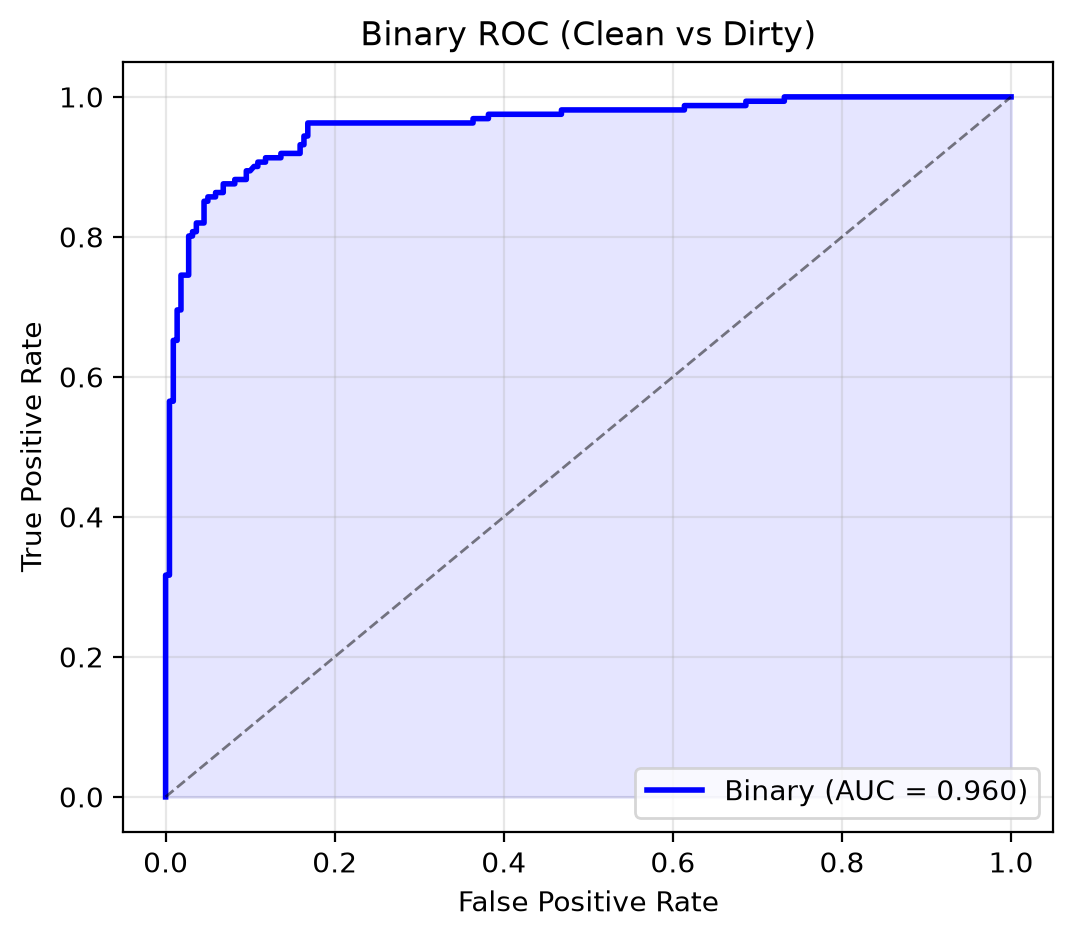
\includegraphics[width=0.9\columnwidth]{figures/fig3_roc_auc.png}
  \caption{Binary ROC curve for clean vs. dirty classification (AUC = 0.9596).}
  \label{fig:roc}
\end{figure}

\begin{figure}[t]
  \centering
  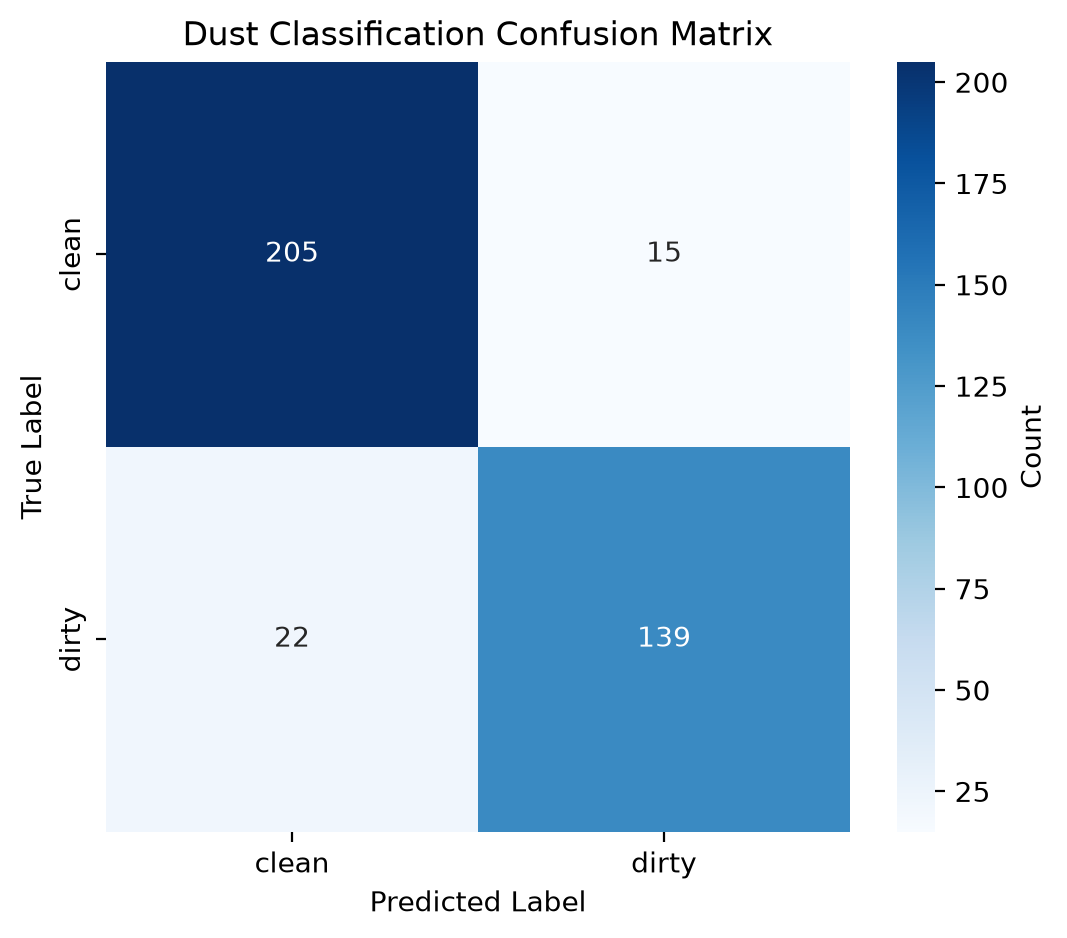
\includegraphics[width=0.9\columnwidth]{figures/fig6_confusion_matrix.png}
  \caption{Confusion matrix for the binary dust-classification task on the test set.}
  \label{fig:confusion}
\end{figure}

\begin{figure}[t]
  \centering
  
\includegraphics[width=0.9\columnwidth]{figures/fig7_confidence.png}
  \caption{Prediction-confidence distribution across test samples.}
  \label{fig:confidence}
\end{figure}

\subsection{Comparison with Existing Approaches and Backbones}
Table~\ref{tab:comparison} compares our framework with published solar dust-detection methods and with the three backbones evaluated in this work. On a binary clean/dirty protocol our EfficientNet-B2 + SVM model (90.29\%, 7.77M params, multi-method XAI) is evaluated on a larger, more diverse multi-source corpus than the literature baselines (SolNet 98.2\% on 2,231 images, Bassil et al. 97\%), while our MobileNetV3-Large + SVM variant (88.71\%, 3.00M params) offers the smallest footprint and ResNet50 + SVM matches the deployed model (90.29\%, 23.59M); all three of our variants exceed Alatwi et al.'s DenseNet-169 + SVM baseline (86.79\%). Reported accuracies are on respective datasets, so the comparison is indicative.

\begin{table}[t]
  \centering
  \caption{Comparison with Existing Methods and Backbone Ablation}
  \label{tab:comparison}
  \begin{tabular}{lccc}
    \toprule
    \textbf{Method} & \textbf{Accuracy} & \textbf{Params} & \textbf{XAI} \\
    \midrule
    SolNet (custom CNN)~\cite{onim2023solnet} & 98.2\% & 56M & -- \\
    DenseNet-169 + SVM~\cite{alatwi2024deep} & 86.79\% & 20M & -- \\
    EffB7 + ViT + tree~\cite{bassil2025efficient} & 97\% & -- & -- \\
    \midrule
    \textbf{Ours (EfficientNet-B2 + SVM)} & \textbf{90.29\%} & \textbf{7.77M} & \textbf{Multi} \\
    \textbf{Ours (MobileNetV3-Large + SVM)} & \textbf{88.71\%} & \textbf{3.00M} & \textbf{Multi} \\
    Ours (ResNet50 + SVM) & 90.29\% & 23.59M & Multi \\
    \bottomrule
  \end{tabular}
\end{table}

\subsection{Cross-Dataset Generalization}
To verify that the detector is not overfit to a single acquisition source, we evaluate the deployed EfficientNet-B2 + SVM model on two \emph{fully independent} external datasets never seen during training. On the 2,562-image binary Dusty/Clean set the model reaches \textbf{98.24\%} accuracy with 98.0\% dirty-class recall, and on the clean/dirty subset of the 6-class faulty-panel set (383 images) it reaches \textbf{99.74\%} accuracy with 100\% dirty-class recall (Table~\ref{tab:external}). The near-perfect external scores confirm that the frozen ImageNet representation plus the SVM head learns source-independent soiling cues rather than dataset-specific artefacts.

\begin{table}[t]
  \centering
  \caption{External Validation on Independent Datasets (deployed EfficientNet-B2 + SVM)}
  \label{tab:external}
  \begin{tabular}{lcc}
    \toprule
    \textbf{External dataset} & \textbf{Accuracy} & \textbf{Dirty recall} \\
    \midrule
    Dusty/Clean (2,562 imgs) & 98.24\% & 98.0\% \\
    Faulty-panel clean/dirty (383 imgs) & 99.74\% & 100\% \\
    \bottomrule
  \end{tabular}
\end{table}

\subsection{XAI Analysis}
We inspect why the hybrid model reaches its decisions using the five methods.

\subsubsection{Grad-CAM Localization}
Grad-CAM heatmaps on the last convolutional block of EfficientNet-B2 weight each spatial feature map by the gradient of the dirty-class score. On clean panels activation spreads broadly across the glass surface, whereas on dirty panels it concentrates on texture-rich, low-contrast regions where soiling is visible (Figure~\ref{fig:gradcam}).

\begin{figure}[t]
  \centering
  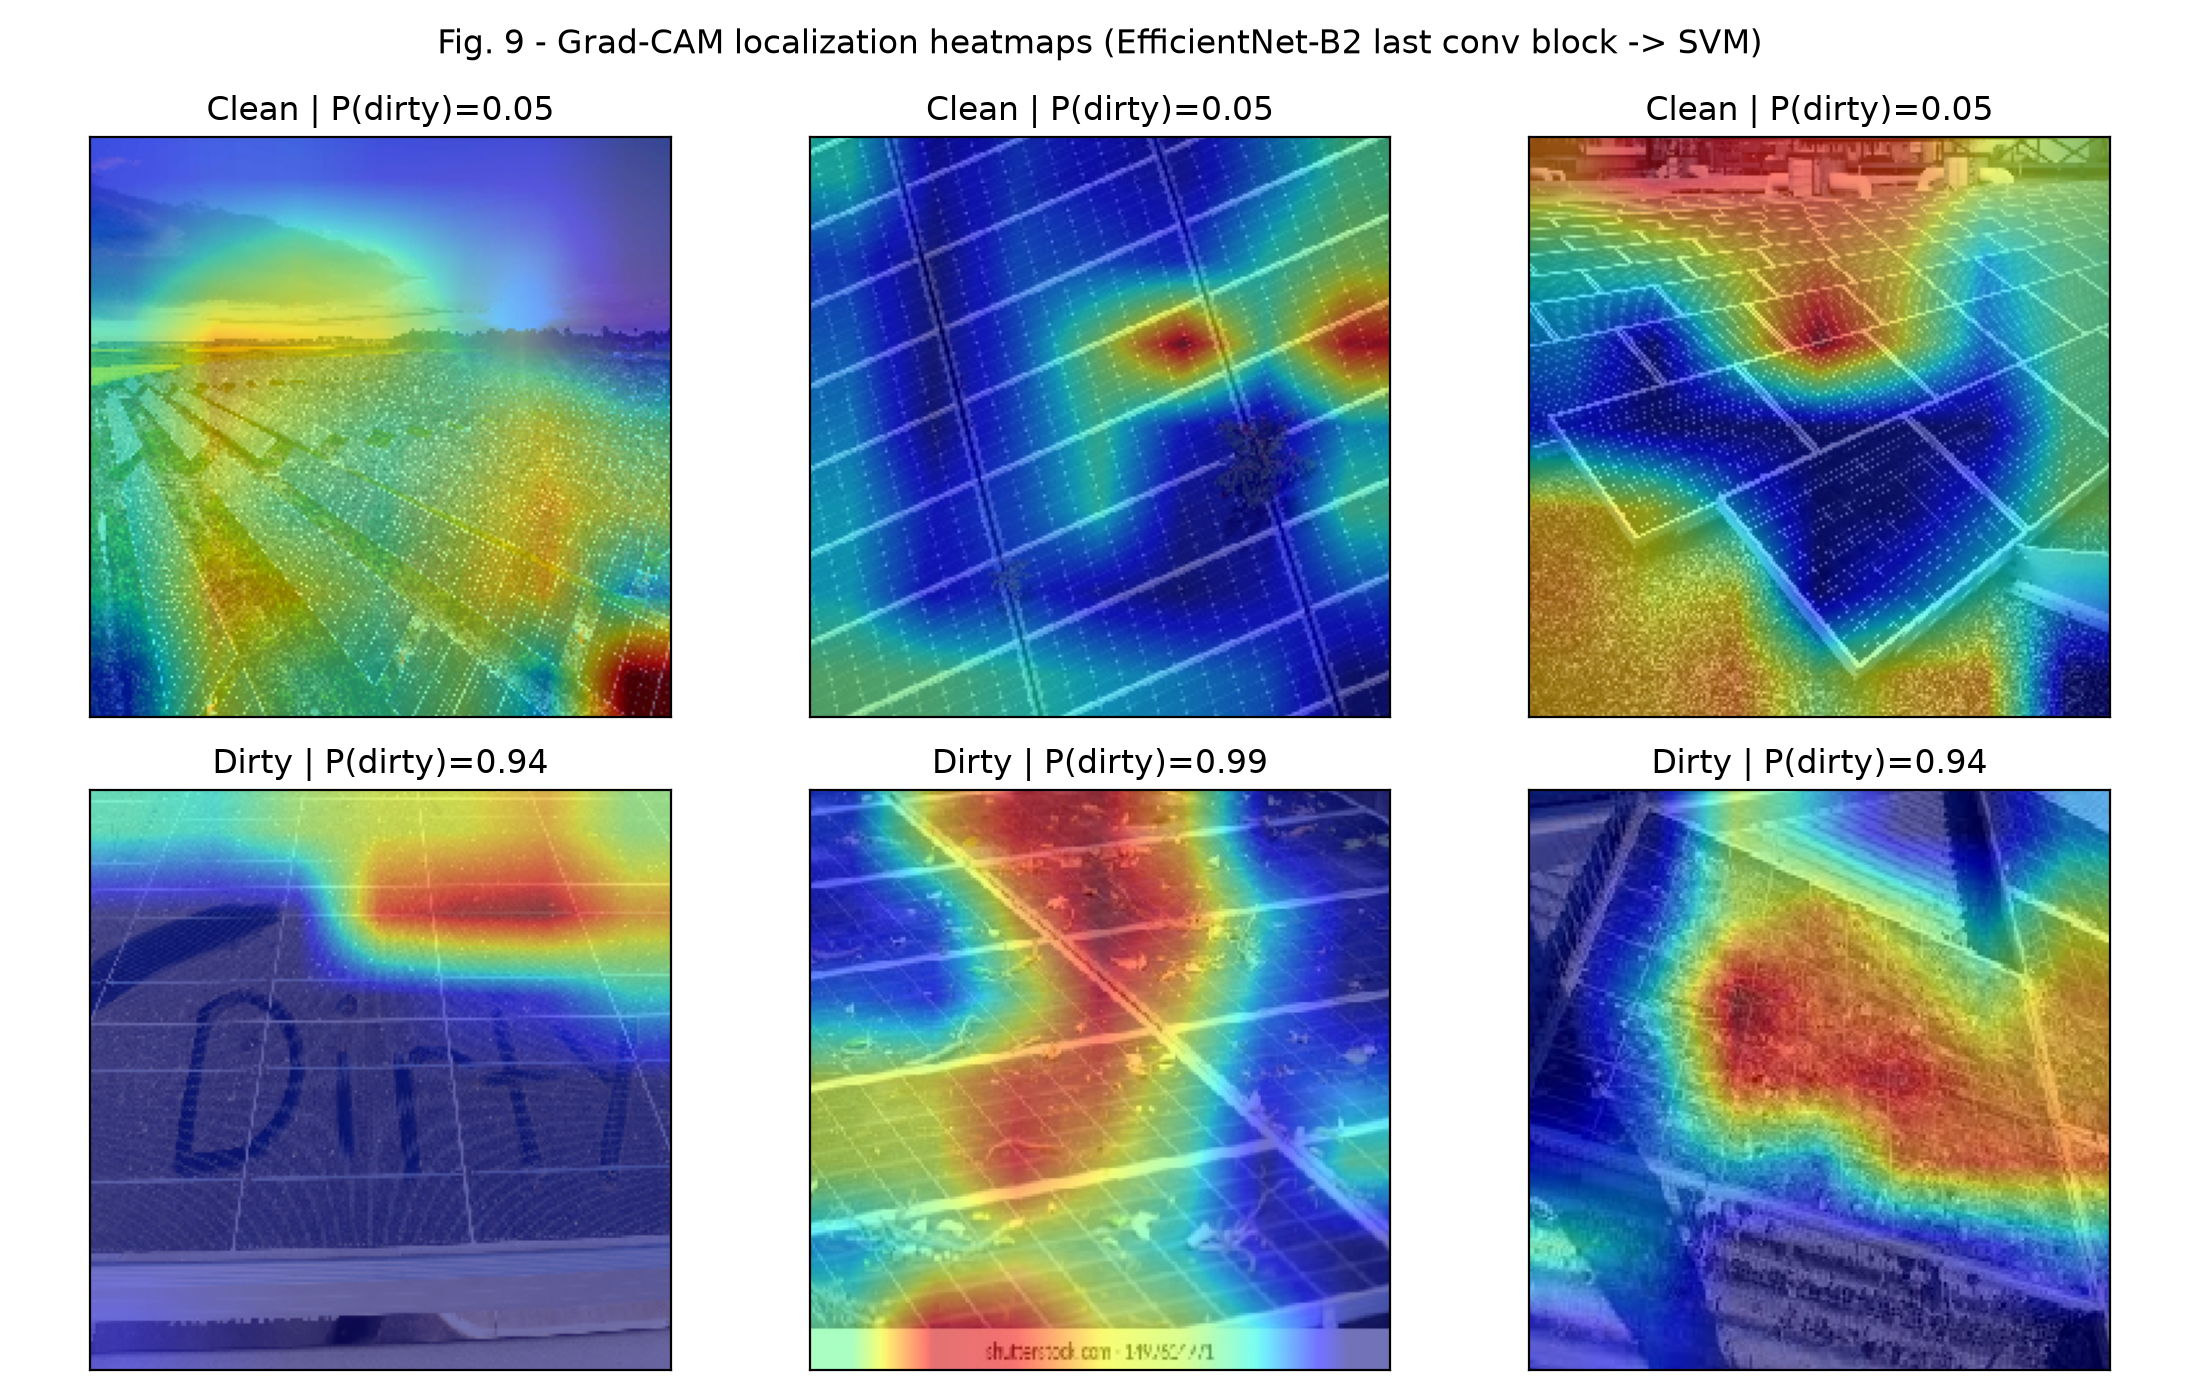
\includegraphics[width=0.9\columnwidth]{figures/fig9_gradcam.png}
  \caption{Grad-CAM localisation heatmaps overlaid on clean and dirty panels, concentrating on soiling-bearing surface regions.}
  \label{fig:gradcam}
\end{figure}

\subsubsection{Score-CAM and Integrated Gradients}
Score-CAM produces gradient-free, high-fidelity localisations, while Integrated Gradients provides pixel-level attributions satisfying the completeness axiom, both confirming that dust-covered texture regions dominate the decision.

\subsubsection{SHAP Feature Analysis}
SHAP applied to the 1,408-dimensional feature vector shows that the top-contributing channels correspond to high-frequency texture filters and low-luminance colour channels, physically consistent with how a uniform dust layer flattens surface texture and attenuates light (Figure~\ref{fig:shap}).

\begin{figure}[t]
  \centering
  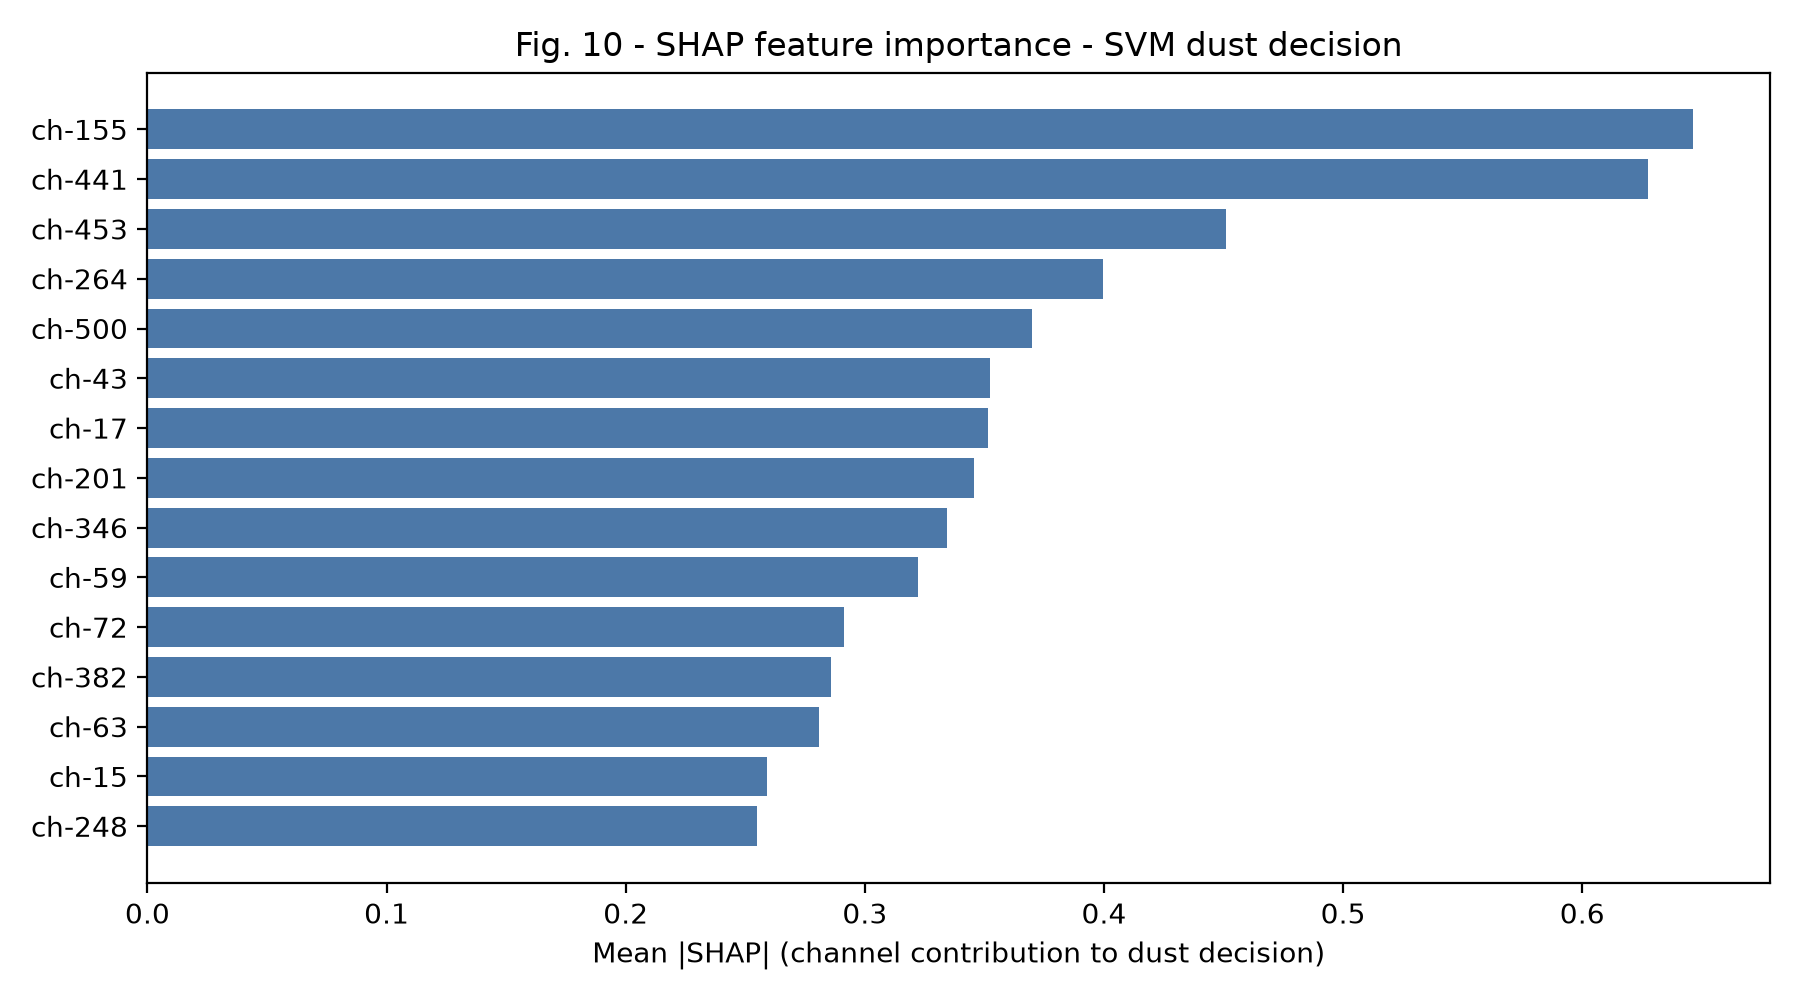
\includegraphics[width=0.9\columnwidth]{figures/fig10_shap.png}
  \caption{SHAP feature importance (top contributing texture and colour channels) for the SVM dust decision.}
  \label{fig:shap}
\end{figure}

\subsubsection{LIME Explanations}
LIME produces sparse, localised explanations that tightly bound dust regions and are interpretable for non-technical operators in the field.

\section{Conclusion}

We presented a hybrid EfficientNet-B2 + SVM framework for binary solar-panel dust detection that achieves 90.29\% test accuracy (0.9596 AUC, 86.38\% CV) on a 3,787-image merged multi-source corpus with only 7.77M parameters, and generalises to two independent external datasets at 98.24\% and 99.74\%; MobileNetV3-Large reaches 88.71\% (3.00M params) at the smallest footprint. A five-method explainability module makes every prediction auditable. Limitations include the per-source dataset sizes and the binary formulation; future work will extend to dust-severity grading, larger multi-site corpora, and TensorFlow-Lite edge deployment for on-panel inference.

\bibliographystyle{plain}
\bibliography{references}

\end{document}
